\chapter{Revisão de literatura}

Como comentado no Capítulo \ref{intro}, modelos matemáticos voltados ao estudo de esportes estão cada vez mais comuns, podendo citar exemplos de modelos voltados ao tênis \cite{bernardo}, hockey no gelo \cite{beaudoin} e basquete \cite{eric}, entre outros. Embora tais esportes sejam distintos, com regras completamente diferentes, alguns elementos de modelagem acabam por se repetir. \cite{beaudoin}, por exemplo, se vale de uma modelagem dada por modelos de Poisson para modelar os gols no hockey, classe de modelos já utilizada por Karlis \cite{karlis2000} \cite{karlis2003} e Lee \cite{lee} para o futebol.

Recentemente, Santos \cite{joao} e Maia \cite{luiz} estudaram modelos matemáticos voltados ao Campeonato Brasileiro. Enquanto Santos comparou os resultados de oito modelos propostos, Maia focou seu estudo na previsão dos resultados in-play, isto é, durante a partida, analisando como as probabilidades de resultado varia conforme o decorrer da partida. Novamente, tais modelos são baseados em modelos de Poisson. 

Os trabalhos supracitados apresentam resultados interessantes ao realizar a modelagem do esporte ao nível de clubes, ou seja, considerando cada uma das partidas como um confronto entre duas ``entidades atômicas''. Cada uma dessas ``entidades'' possuí alguma força estimada por meio dos dados observados, o que possibilita a modelagem e a comparação entre os clubes. Entretanto, como os clubes são formados por um conjunto de jogadores, é natural pensar na modelagem a nível individual, agora considerando cada jogador como uma ``entidade atômica'' para o modelo.

Partindo para a modelagem individual, Wolf \cite{wolf} propõe um ranqueamento baseado no algoritmo Elo, proposto por Arpad Emrick Elo (1903 - 1992) nos anos 60 e utilizado até hoje pela FIDE. Para a modelagem, Wolf se vale dos dados de 18 competições europeias das temporadas 14/15 a 17/18. Os resultados desse artigo são interessantes, trazendo tanto o ranqueamento dos jogadores como também qual o impacto de cada jogador para seu clube.

Para o presente trabalho o objetivo é misturar algumas das ideias acima, realizando a modelagem do futebol brasileiro por meio de modelos de Poisson, mas a nível individual. Tal objetivo visa analisar o desempenho da modelagem de jogadores em relação a modelagem de clubes, além de possibilitar uma melhor interpretabilidade na predição de resultados para o futebol em relação a predição obtida com o algoritmo Elo.

\chapter{Aquisição dos dados}
\label{aquisicao}

Tendo em vista os modelos abordados no capítulo anterior, bem como o escopo idealizado para o trabalho, o primeiro passo se dá pela aquisição dos dados. Com isso em mente, esse capítulo visa mostrar como ocorreu tal processo.

\section{Processo de raspagem}

Como etapa inicial, realizou-se a extração dos dados dos jogos realizados em torneios da CBF \cite{cbf} entre os anos de 2013 e 2022. O processo de raspagem dos dados foi realizado em Python, dentro de um servidor Linux, e dividido em três etapas.

A primeira etapa se refere a extração da informação propriamente dita, sendo utilizadas, principalmente, as bibliotecas \path{requests} e \path{PyPDF2}. Nessa etapa, a ideia era a de extrair as súmulas, em PDF, do site da CBF e convertê-las para \path{csv}. Como as súmulas já seriam acessadas e armazenadas, temporariamente, na máquina local, optou-se por guardá-las para identificação e correção de possíveis erros na próxima etapa da raspagem.

A segunda etapa, iniciada após a conversão das súmulas para \path{csv}, consistiu na extração das informações de cada jogo: times, resultado final, jogadores relacionados, gols e substituições. Por questões de simplicidade, as expulsões não foram coletadas. Ao final dessa etapa, as informações de cada campeonato, separadas por ano, foram convertidas para \path{json}, sendo codificadas pelo número do jogo, que pode ser encontrado na própria súmula. Como exemplo, a Listing \ref{exemplo_json1} mostra como o primeiro jogo de 2022, entre Atlético Mineiro e Internacional, foi armazenado.
\begin{lstlisting}[language = json, firstnumber = 1, caption = {Exemplo de JSON obtido após a segunda etapa.}, captionpos = b, label = exemplo_json1]
{
  "001": {
    "Mandante": "Atletico Mineiro / MG",
    "Visitante": "Internacional / RS",
    "Resultado": "2 X 0",
    "Jogadores": [
      [
        "22Everson Everson Felipe Marqu ... T(g)P188398",
        "Atletico Mineiro / MG"
      ],
      [
        "2Guga Claudio Rodrigues Gomes TP317445",
        "Atletico Mineiro / MG"
      ],
      ],
      ...,
      [
        "1Daniel Daniel de Sousa Brito T(g)P331033",
        "Internacional / RS"
      ],
      [
        "3Kaique Kaique Rocha Lima TP442170",
        "Internacional / RS"
      ],
      ...
    ],
    "Gols": [
      "09:00 1T 7 NR Givanildo Vieira de Sousa Atletico Mineiro/MG",
      "+2 2T 7 NR Givanildo Vieira de Sousa Atletico Mineiro/MG"
    ],
    "Substituicoes": [
      "45:00 INT Internacional/RS 25 - Gabriel Ivan Mercado 9 - Wesley Moraes Ferreira da Si...",
      "12:00 2TAtletico Mineiro/MG 15 - Federico Matias Zaracho 18 - Eduardo Colcenti Antunes",
      "19:00 2TAtletico Mineiro/MG 8 - Jair Rodrigues Junior 5 - Otavio Henrique Passos Santos",
      "19:00 2TAtletico Mineiro/MG 17 - Jefferson David Savarino Qui... 19 - Ademir da Silva Santos Junior",
      "20:00 2TInternacional/RS 35 - Alexandre Zurawski 27 - Mauricio Magalhaes Prado",
      "33:00 2TAtletico Mineiro/MG 10 - Eduardo Jesus Vargas Rojas 11 - Marcos da Silva Franca",
      "34:00 2TInternacional/RS 21 - Gabriel Boschilia 5 - Igor Matheus Liziero Pereira",
      "43:00 2TInternacional/RS 47 - Caio Vidal Rocha 22 - Bruno Mendez Cittadini"
    ]
  }
}
\end{lstlisting}

Tendo concluído a segunda etapa, partiu-se para a montagem das escalações de cada um dos jogos. Para tanto, os jogadores foram identificados por seu código CBF. Nessa etapa, além da escalação inicial (os vinte e dois atletas que iniciaram a partida), foram montadas escalações secundárias, de modo que cada uma das escalações representasse um momento da partida, isso é, o período entre uma substituição e outra. Assim, a primeira escalação se deu pelos times que entraram em campo, enquanto as demais foram elaboradas seguindo as próprias alterações da partida, removendo o jogador que foi substituído e incluindo o atleta que entrou em campo. Para substituições que ocorrem no mesmo minuto, como a entrada de Jair e Jefferson para a saída de Otávio e Ademir, pelo Atlético Mineiro, observada na Listing \ref{exemplo_json1}, foi considerada apenas uma nova escalação.

Consequentemente, com essa quebra do jogo em função das escalações, o tempo de jogo e o placar também foram adaptados para coincidir com o intervalo de jogo que a escalação atual se refere. Com o objetivo de ilustrar essa ideia, a Listing \ref{exemplo_json2} traz o início do arquivo das escalações, mostrando as escalações elaboradas para o jogo citado previamente. Novamente, o primeiro indexador do arquivo é o código do jogo, dado pela CBF, e o segundo pode ser interpretado como o número de paradas para substituição de jogadores que ocorreram até o início daquela escalação.
\begin{lstlisting}[language = json, firstnumber = 1, caption = {Exemplo do JSON final.}, captionpos = b, label = exemplo_json2]
{
  "001": {
    "0": {
      "Mandante": [
        "188398", "317445", "699115", "320930", "163056", "375634", "339258", "295792", "438212", "339266", "370997"
      ],
      "Visitante": [
        "331033", "442170", "344934", "177042", "306270", "387944", "756803", "750897", "648335", "320839", "542337"
      ],
      "Tempo": 45,
      "Placar": [
        1,
        0
      ]
    },
    "1": {
      "Mandante": [
        "188398", "317445", "699115", "320930", "163056", "375634", "339258", "295792", "438212", "339266", "370997"
      ],
      "Visitante": [
        "331033", "442170", "344934", "177042", "306270", "756803", "750897", "648335", "320839", "542337", "723593"
      ],
      "Tempo": 12,
      "Placar": [
        0,
        0
      ]
    },
    "2": {
      "Mandante": [
        "188398", "317445", "699115", "320930", "163056", "375634", "339258", "438212", "339266", "370997", "703937"
      ],
      "Visitante": [
        "331033", "442170", "344934", "177042", "306270", "756803", "750897", "648335", "320839", "542337", "723593"
      ],
      "Tempo": 7,
      "Placar": [
        0,
        0
      ],
      ...
    }
  }
}
\end{lstlisting}

Como comentado anteriormente, os tempos de jogo e gols também foram adaptados para a quebra das escalações. Dessa forma, note que, pela Listing \ref{exemplo_json1}, podemos ver que o Internacional sofreu um gol no primeiro tempo e que realizou uma substituição no intervalo, sendo a primeira substituição do jogo. Esses dois eventos se refletem na Listing \ref{exemplo_json2} com a primeira escalação (indexada pelo 0), tendo o placar de 1x0 e tempo total de 45 minutos. Como aos 12 minutos do segundo tempo o Atlético fez uma alteração, a escalação indexada pelo 1 possui 12 minutos de duração e placar igual a 0x0, pois não houveram gols nesse período. As demais escalações foram definidas de modo análogo, com o tempo de jogo limitado a 90 minutos e, todos os eventos que ocorreram durante os acréscimos, levados para o último minuto do respectivo tempo de jogo.

\section{Problemas durante a raspagem}

Durante a raspagem algumas súmulas fugiram do padrão, principalmente as que se referiam do período de 2013 a 2016. Algumas em virtude de W.O., outras com preenchimento incorreto. Os erros mais básicos, como o W.O. e a falta da unidade federativa no nome de alguns times, foram tratados de forma semi-manual e colocados em um arquivo \path{json} de exceções. Tendo resolvido tais problemas, a transição da primeira para a segunda etapa foi concluída, restando, portanto, apenas a outra transição.

Mais uma vez, durante o caminho da segunda para a terceira etapa foram evidenciados alguns erros, principalmente no preenchimento das súmulas, com informações que não faziam sentido. Em virtude disso, tais erros foram tratados, predominantemente, de forma manual. A opção pelo tratamento manual, apesar de trabalhosa, se deu pelo fato de que existiam erros que necessitavam de verificação externa para validar (ou até mesmo coletar) a informação correta.

Um exemplo de como tais erros ocorreram pode ser visto nas Figuras \ref{erro_ext1} e \ref{erro_ext2}. Note que o jogador Centurión, do São Paulo, foi, de acordo com a súmula, relacionado como titular. Entretanto, aos 24 minutos do segundo tempo ele é chamado para entrar em campo substituindo o camisa 25, Hudson.

Outro jogador, na mesma partida, também teve sua participação documentada de forma incorreta. O camisa 11, Alexandre Pato, foi relacionado como reserva. Entretanto, aos 29 minutos do segundo tempo, o mesmo deixa o campo para a entrada de Thiago Henrique, camisa 23, sendo que, pela súmula, o camisa 11 nem teria entrado em campo previamente.

Esses erros, envolvendo a escalação inicial do clube, foram recorrentes, com mais jogos apresentando situações similares.
\begin{figure}[H]
    \centering
    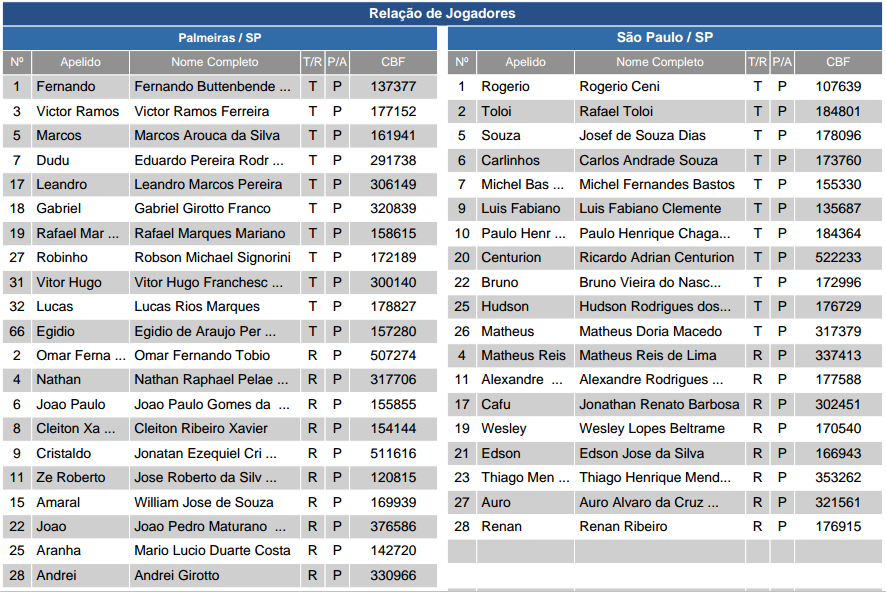
\includegraphics[scale = 0.5]{palmeiras_sao_paulo_2015_jogadores.png}
    \caption{Relação de jogadores da partida entre Palmeiras e São Paulo pela Série A de 2015.}
    \label{erro_ext1}
\end{figure}

\begin{figure}[H]
    \centering
    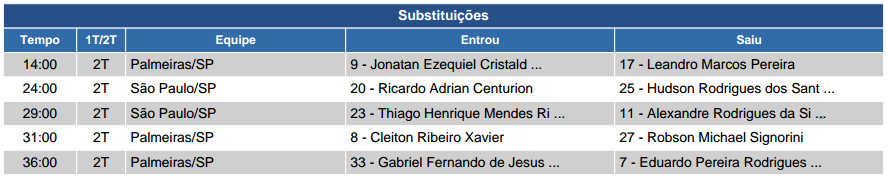
\includegraphics[scale = 0.5]{palmeiras_sao_paulo_2015_substituicoes.png}
    \caption{Substituições da partida entre Palmeiras e São Paulo pela Série A de 2015.}
    \label{erro_ext2}
\end{figure}

Além dos erros de preenchimento do time titular, outro erro comum foi no preenchimento das substituições, como pode ser visto na Figura \ref{erro_ext3}. Nela o mesmo jogador, João Rodrigues, entrou e deixou o campo no mesmo minuto. O problema, nesse caso, se deu pelo fato dele primeiro sair de campo para, depois, entrar.
\begin{figure}[H]
    \centering
    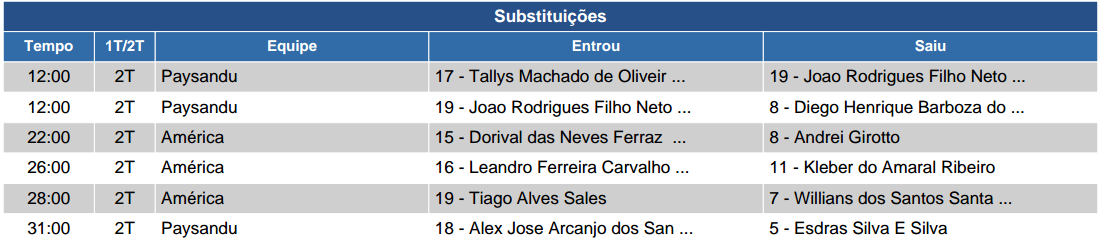
\includegraphics[scale = 0.4]{paysandu_america_2013.png}
    \caption{Relação de jogadores da partida entre Paysandu e América pela Série B de 2013.}
    \label{erro_ext3}
\end{figure}

Tais erros foram corrigidos manualmente, e, por simplicidade, foram alterados diretamente nos arquivos \path{csv} gerados na primeira etapa. Dessa forma, ao executar o processo de raspagem, a segunda etapa da extração corrige os jogos com erros nos arquivos \path{json} e, com isso, a passagem da segunda etapa para a terceira está corrigida.

\section{Automação do processo}

Durante o desenvolvimento do trabalho muitos campeonatos de 2022 ainda estavam em andamento, logo a extração de dados deveria, idealmente, ser constante. Aliando isso com o fato de que, no momento em que o código da raspagem foi finalizado, nenhum jogo dos últimos anos apresentou problema ao extrair as informações, poderíamos apenas executar o código da raspagem dos dados com certa frequência. Pensando em evitar que essa rotina fosse realizada de forma manual foi criado, no GitHub Actions, uma rotina para que todo dia a raspagem fosse executada. Essa rotina englobou todo o processo de raspagem, desde a coleta das súmulas até os tratamentos das etapas finais, onde o arquivo \path{json} é elaborado.

Nesse ponto, com o intuito de poupar custos computacionais, vale ressaltar que os arquivos finais só eram regerados no caso em que havia a inclusão de um novo jogo na base ou a alteração de algum jogo já existente. Tal regra foi criada pois se não houvesse nenhuma alteração nos dados da base as informações a serem coletadas deveriam ser, necessariamente, as mesmas.

Como o processo de raspagem requer conexão com a internet, foi elaborado um gatilho para parar a execução pois, a depender da rede, a conexão poderia demorar. Nesse sentido, foram utilizadas as bibliotecas \path{multiprocessing} e \path{time} para limitar o tempo de raspagem de cada competição, encerrando o processo caso o tempo total de extração, de uma temporada, ultrapasse dois minutos. A escolha de tal tempo foi dada em virtude de que, como a rotina é diária, o maior número de jogos que seriam coletados em um dia, para uma competição, ocorreria no caso de rodada cheia, com 10 jogos.

Entretanto, caso o tempo do processo tenha ultrapassado esse limite, mas tenham sido adicionados novos jogos, o processo de raspagem é repetido, evitando que, no caso de uma raspagem em massa (do campeonato inteiro, por exemplo), algum jogo não seja coletado em virtude da expiração do tempo.

Por fim, para acompanhamento desse processo, foi elaborado um arquivo de log, onde, como pode-se ver na Figura \ref{log}, traz as informações gerais sobre o número de jogos adicionados, além de informar caso algum jogo tenha gerado algum erro.
\begin{figure}
    \centering
    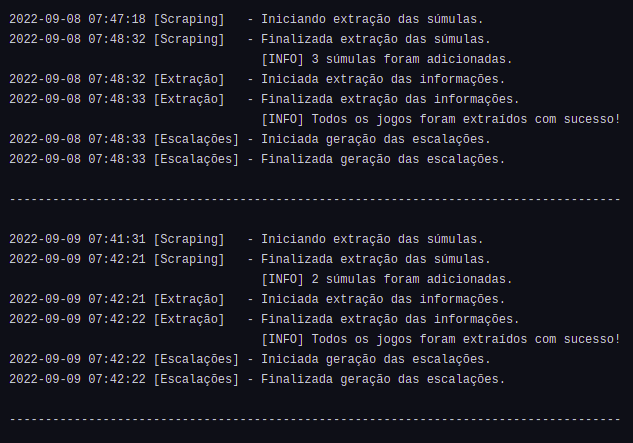
\includegraphics[scale = 0.6]{log.png}
    \caption{Log do processo de raspagem.}
    \label{log}
\end{figure}

\chapter{Modelagem proposta}

\section{Premissas utilizadas}
\label{premissas}

Assim como utilizado por outros autores (\cite{beaudoin}, \cite{karlis2000}, \cite{karlis2003}, \cite{lee}, entre outros), estaremos considerando que os gols em uma partida de futebol seguem uma distribuição de Poisson. Para dar mais credibilidade a premissa, podemos ver, na Figura \ref{goals_graph}, a distribuição de gols por partida, separada em mandante e visitante, para todo período extraído. Para comparar com a distribuição de Poisson, plotou-se juntamente do histograma de gols, a função de massa de probabilidade da Poisson de máxima verossimilhança dos dados observados, isso é, onde $\lambda_m = \frac{1}{|G|}\sum_{g \in G} s_{m, g}$ e $\lambda_v = \frac{1}{|G|}\sum_{g \in G} s_{v, g}$.
\begin{figure}[h]
    \centering
    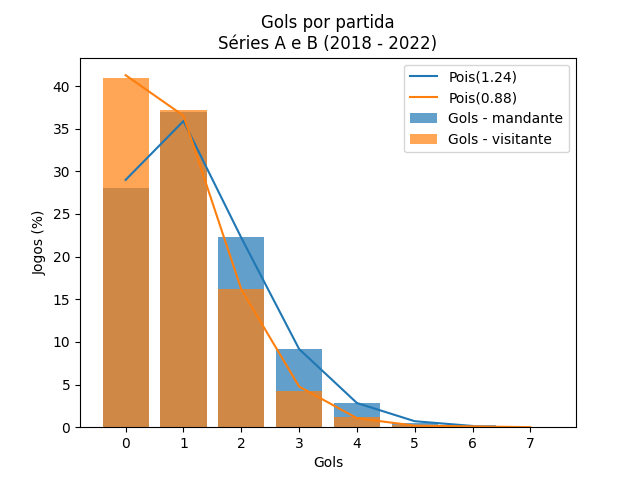
\includegraphics[scale = 0.8]{goals.png}
    \caption{Histograma de gols por partida.}
    \label{goals_graph}
\end{figure}

Conforme podemos ver na Figura \ref{goals_graph}, as duas distribuições (gols marcados na partida e Poisson) são bem similares, embora isso não assegure que podemos afirmar que os dados vêm de uma distribuição de Poisson. Para testar essa hipótese podemos realizar um Teste $\chi^2$ de Aderência (ou teste de Bondade do Ajuste) \cite{gof}. Esse teste pode ser utilizado com o objetivo de testar a hipótese $H_0$, de que o conjunto de dados observados segue uma determinada distribuição, contra a hipótese $H_a$, de que o conjunto de dados observados não é oriundo dessa distribuição. A estatística a ser testada é dada por
\begin{equation}
    \Lambda = \sum_{i \in \mathbb{Z}_+} \mathbb{1}_{O_i \neq 0} \dfrac{\left(O_i - E_i\right)^2}{E_i},
    \label{lambda_teste}
\end{equation}

\noindent onde $\mathbb{1}_{O_i \neq 0}$ é a função indicadora, valendo $0$ se $O_i = 0$ e $1$ caso contrário, $O_i$ é o número de jogos em que o time analisado marcou $i$ gols e $E_i$ é o número esperado, segundo a distribuição de $H_0$ do número de jogos em que o time analisado marcaria $i$ gols.

Tal estatística segue uma distribuição $\chi^2_{k - 2}$ sendo,
\[k = \sum_{i \in \mathbb{Z}_+} \mathbb{1}_{O_i \neq 0}.\]

Por fim, $H_0$ é rejeitada caso $\Lambda > \chi^2_{1 - \alpha, k - 2}$, onde $\alpha$ é nível do teste e $\chi^2_{1 - \alpha, k - 2}$ é o valor crítico para o teste.

Todas as contas do teste foram realizadas em Python. Utilizando $\alpha = 0.05$, chegamos nos resultados da Tabela \ref{hyp_test}. Ambos os testes falharam em rejeitar a hipótese nula, de que os dados observados seguem a distribuição de Poisson vista na Figura \ref{goals_graph}.
\begin{table}[h]
    \centering
    \begin{tabular}{|r|c|c|}
        \hline
        Distribuição & $\Lambda$  & Valor Crítico \\ \hline
        Mandante     & 7.0253     & 11.0705       \\
        Visitante    & 10.4619    & 11.0705       \\ \hline
    \end{tabular}
    \caption{Resultados do teste de Bondade do Ajuste.}
    \label{hyp_test}
\end{table}

Outra premissa muito importante, imposta por questões de simplicidade, é a de que os jogadores são independentes. Dessa forma, as escalações dos dois clubes são independentes e, dentro de um mesmo clube, não existem jogadores com mais ou menos entrosamento entre si. Isso é, não estamos considerando as possibilidade de haver um racha no elenco ou um grande entrosamento entre dois jogadores. Também por questões de simplicidade, não estaremos considerando o cansaço dos jogadores, assim os jogadores mantém seu rendimento igual por toda a partida. Abordaremos mais a fundo essas premissas na Subseção \ref{selecao_de_dados}.

Por fim, como comentado brevemente no capítulo anterior, estaremos supondo que todas as partidas são independentes entre si e possuem, exatamente, 90 minutos. Além disso, todos os eventos ocorridos durante os acréscimos são considerados como se tivessem ocorrido no minuto imediatamente anterior (45 minutos do primeiro ou do segundo tempo). Tal suposição se dá pelo próprio processo de raspagem, no qual não foram considerados os acréscimos, jogando todos os eventos dos mesmos para o último minuto da etapa atual do jogo.

\section{Tratamento e Seleção dos dados}

Tendo em mãos os dados para serem utilizados e as premissas, o próximo passo é, naturalmente, a seleção dos dados que irão entrar no modelo.

\subsection{Tratamento dos dados}
\label{tratamento_dos_dados}

Como estamos modelando as partidas em função dos jogadores que estão em campo, sempre que ocorre uma substituição todo o contexto muda, uma vez que, pelo menos, um clube mudou. Desse modo, para modelar esse fenômeno podemos redefinir as partidas, quebrando-as em subpartidas correspondentes a cada substituição. Dessa forma, uma partida $g$ com $n_g$ substituições será quebrada em $n_g + 1$ partidas, de modo que cada intervalo de quebra represente os eventos que ocorreram naquele intervalo. Tal quebra já foi relatada na Seção \ref{aquisicao}, além de ter sido implementada no processo de raspagem. Naturalmente, devemos ter
\[\sum_{k = 0}^{n_g} t_{g, k} = 90,\]
\[\sum_{k = 0}^{n_g} s_{m, g, k} = s_{m, g} \text{ e}\]
\[\sum_{k = 0}^{n_g} s_{v, g, k} = s_{v, g}.\]

\begin{mybox}{gray}{Exemplo 1}
    Em uma partida hipotética $g$ na qual ocorreram $3$ substituições, uma aos $29'$, outra aos $57'$ e outra aos $62'$, com gols aos $11'$ para o mandante e aos $87'$ para o visitante terá as seguintes características:
    \begin{table}[H]
        \centering
        \begin{tabular}{r|l}
            Nome & Valor \\ \hline
            $n_g$ & $3$ \\
            $t_{g, 0}$ & $29$ \\
            $s_{g, m, 0}$ & $1$ \\
            $s_{g, v, 0}$ & $0$ \\
            $t_{g, 1}$ & $28$ \\
            $s_{g, m, 1}$ & $0$ \\
            $s_{g, v, 1}$ & $0$ \\
            $t_{g, 2}$ & $5$ \\
            $s_{g, m, 2}$ & $0$ \\
            $s_{g, v, 2}$ & $0$ \\
            $t_{g, 3}$ & $28$ \\
            $s_{g, m, 3}$ & $0$ \\
            $s_{g, v, 3}$ & $1$ \\
            $s_{g, m}$ & $1$ \\
            $s_{g, v}$ & $1$
        \end{tabular}
    \end{table}
\end{mybox}

Com tais substituições, as forças gerais dos dois clubes acabam se alterando conforme o jogo acontece e os jogadores são substituídos, o que faz com que surjam os conjuntos de jogadores a cada período de jogo\footnote{Cada período sendo dado no intervalo de tempo entre substituições ou início/término da partida.} e, consequentemente, as forças de ataque e defesa de cada clube para cada período de tempo.

\subsection{Seleção dos dados}
\label{selecao_de_dados}

O objetivo do trabalho é a modelagem do futebol brasileiro atual. Assim, para a modelagem, iremos nos valer dos dados mais recentes possíveis e sempre das divisões superiores. Nesse sentido, a preferência sempre será dada a jogos das Séries A e B, com os anos mais recentes.

Pelo fato dos clubes das Séries C e D não enfrentarem todos os outros clubes de sua divisão, os dados dessas duas divisões não serão utilizados, uma vez que isso pode dificultar a modelagem de alguns jogadores, além de aumentar a complexidade do modelo. Já os dados da Copa do Brasil serão deixados de lado visando evitar os clubes das Séries C e D que jogam tal competição e, principalmente, em razão da complexidade do modelo. Assim, os dados que serão utilizados tratam das equipes das Série A e, talvez, B, restando definir o período que será considerado.

Para melhor escolha dos dados, a Tabela \ref{dados_totais} apresenta a quantidade geral de jogadores e subpartidas que forem coletados. Como explicado anteriormente, queremos focar nos dados mais recentes de, no máximo, duas divisões do campeonato brasileiro (Séries A e B). Dessa forma, as tabelas foram organizadas de modo que os valores se acumulam à medida que avancemos para baixo e para a direita. Ou seja, o valor 3429 da primeira tabela, na linha correspondente ao ano de 2017 e da coluna correspondente a Série B significa que 3429 jogadores entraram em campo em jogos das Séries A e B entre os anos de 2017 e 2022.
\begin{table}[h]
    \centering
    \begin{tabular}{l|rr}
        \hline
         Ano &   Série A &   Série B \\ \hline
        2022 &       747 &      1501 \\
        2021 &      1048 &      1978 \\
        2020 &      1289 &      2415 \\
        2019 &      1531 &      2801 \\
        2018 &      1765 &      3154 \\
        2017 &      1982 &      3496 \\
        2016 &      2213 &      3901 \\
        2015 &      2415 &      4287 \\
        2014 &      2648 &      4709 \\
        2013 &      2851 &      5090 \\
    \hline
    \end{tabular}
    \hspace{50pt}
    \begin{tabular}{l|rr}
        \hline
         Ano &   Série A &   Série B \\ \hline
        2022 &      2506 &      5059 \\
        2021 &      4978 &     10048 \\
        2020 &      7500 &     15112 \\
        2019 &      9864 &     19901 \\
        2018 &     12266 &     24725 \\
        2017 &     14637 &     29487 \\
        2016 &     16982 &     34224 \\
        2015 &     19377 &     39005 \\
        2014 &     21726 &     43711 \\
        2013 &     24064 &     48452 \\
        \hline
    \end{tabular}
    \caption{Dados totais. À esquerda referente ao número de jogadores, à direita referente ao total de subpartidas.}
    \label{dados_totais}
\end{table}

Com os dados da Tabela \ref{dados_totais} podemos voltar a discussão iniciada na Seção \ref{premissas}, sobre a independência dos jogadores. Se considerarmos que os jogadores possuem influência um sobre o outro, devemos ter, na pior das hipóteses, para cada par de jogadores um parâmetro que represente essa influência. Tal parâmetro deve agir de modo que aumente (ou diminua) as chances de um clube marcar gol. Um exemplo simples de como isso funcionaria seria pensar em um atacante e um goleiro que, em algum momento do passado, foram companheiros de time, treinando e jogando juntos. Naturalmente o goleiro irá conhecer o atacante e vice-versa, o que possibilitaria a adoção de alguma estratégia (individual ou coletiva), para neutralizar ou explorar o adversário.

Nesse sentido, a dependência dos jogadores parece ser favorável a modelagem, ao menos na tarefa de tentar prever resultados. Porém, pela Tabela \ref{jogadores_correlacionados}, que mostra a quantidade de pares de jogadores que estavam em campo simultaneamente, podemos ver que a inclusão de algum parâmetro que correlacione os jogadores deixa o modelo demasiadamente complexo. Além disso, o modelo fica inviabilizado, uma vez que o número de pares de jogadores supera, em muito, o número de subpartidas, dadas na Tabela \ref{dados_totais}. Logo, além de simplificar a modelagem, a premissa da independência dos jogadores possibilita a realização da mesma.
\begin{table}[H]
    \centering
    \begin{tabular}{l|rr}
        \hline
         Ano &   Série A &   Série B \\ \hline
        2022 &     82841 &    169001 \\
        2021 &    144390 &    225203 \\
        2020 &    201045 &    284071 \\
        2019 &    249634 &    318987 \\
        2018 &    298906 &    368844 \\
        2017 &    345388 &    413307 \\
        2016 &    393498 &    463228 \\
        2015 &    439449 &    509984 \\
        2014 &    487534 &    558736 \\
        2013 &    532641 &    602980 \\
    \hline
    \end{tabular}
    \caption{Número de pares de jogadores que estiveram em campo simultaneamente.}
    \label{jogadores_correlacionados}
\end{table}

Por fim, por meio da observação da Tabela \ref{dados_totais} e por testes em relação aos limites computacionais, optou-se pela utilização dos dados das Séries A e B, a partir de 2018.

\section{Abordagem Frequentista}
\label{abordagem_frequentista}

Como visto ao final da Seção \ref{tratamento_dos_dados}, as forças de ataque e defesa dos clubes, em cada período de um jogo, irão variar, sendo dadas, em cada subpartida, pelas equações em \ref{lambdas}.
\begin{equation}
    \begin{split}
        \lambda_{m, a, g, k} & = \sum_{i \in \mathcal{C}_{m, g, k}} p_{i, a}, \\
        \lambda_{v, a, g, k} & = \sum_{i \in \mathcal{C}_{v, g, k}} p_{i, a}, \\
        \lambda_{m, d, g, k} & = \sum_{i \in \mathcal{C}_{m, g, k}} p_{i, d} \text{ e} \\
        \lambda_{v, d, g, k} & = \sum_{i \in \mathcal{C}_{v, g, k}} p_{i, d},
    \end{split}
    \label{lambdas}
\end{equation}

\noindent onde $p_{i, a}$ e $p_{i, d}$ representam, respectivamente, as proficiências de ataque e de defesa do jogador $i$. Notemos que aqui não faz sentido que tais parâmetros sejam negativos, uma vez que, nesse caso, a escalação de um jogador pioraria o desempenho do time. Por fim, a média da distribuição de Poisson será dado pelo produto do tempo da subpartida e a razão entre a força de ataque de um clube e a força de defesa do outro, o que representa a taxa de espera entre gols. Em termos matemáticos, podemos expressar o modelo como em \ref{ADM_model}.
\begin{equation}
    \begin{split}
    s_{m, g, k} & \sim \operatorname{Poisson}\left(\dfrac{\lambda_{m,a,g,k}}{\lambda_{v,d,g,k}} \cdot t_{g,k}\right) \\
    s_{v, g, k} & \sim \operatorname{Poisson}\left(\dfrac{\lambda_{v,a,g,k}}{\lambda_{m,d,g,k}} \cdot t_{g,k}\right).
    \end{split}
    \label{ADM_model}
\end{equation}

Notemos que o modelo dado pelas equações em \ref{ADM_model} possui um problema de identificabilidade. Dado o conjunto de parâmetros $\mathcal{P}$, o conjunto $\mathcal{P}' = c\cdot \mathcal{P}$, definido por meio da multiplicação de cada parâmetro por $c$, o modelo que se vale do conjunto $\mathcal{P}'$ é idêntico ao modelo que usa o conjunto $\mathcal{P}$. Essa equivalência ocorre pelo fato do fator $c$ ser simplificado no cálculo do parâmetro de cada uma das distribuições. Para tratar tal problema, fixou-se o primeiro parâmetro do modelo como sendo igual a $1$, isso é, o parâmetro de ataque do primeiro jogador do modelo será fixo.

Agora, com o modelo definido e o problema de identificabilidade tratado, podemos iniciar o processo de modelagem. Como no contexto frequentista o objetivo é o de estimar os parâmetros que, dadas as partidas observadas, maximizam a verossimilhança do processo como um todo, devemos, primeiramente, encontrar a função de verossimilhança.

Por se tratar de várias subpartidas independentes, a verossimilhança se dá por um produtório de vários termos. Entretanto, todos esses termos podem ser interpretados como uma probabilidade, ou seja, estão em $[0, 1]$ ou, quase certamente, em $(0, 1)$. Com isso, computacionalmente, poderíamos ter problemas com ponto flutuante conforme o produtório é realizado, de modo que podemos obter um valor muito baixo, sendo impossível de representar o mesmo computacionalmente. O tratamento clássico para tal problema é a aplicação do logaritmo que, por ser uma função monótona, não afeta o processo de otimização, isso é, como temos que $x < y \implies \log{x} < \log{y}$, se $x$ é o valor ótimo da verossimilhança, $\log{x}$ será o valor ótimo da função de log-verossimilhança.

Além de tratar o problema de ponto flutuante, a aplicação do log faz com que os produtórios sejam reescritos como somatórios, o que também auxilia no tratamento do problema a nível computacional. Diante do exposto, podemos escrever a função de log-verossimilhança dos dados, conforme Equação \ref{log_vero}.
\begin{equation}
    \begin{split}
        \mathcal{L}(p_a, p_d | G) & = \sum_{g}\sum_{k = 0}^{n_g}\left(-\dfrac{\lambda_{m, a, g, k}}{\lambda_{v, d, g, k}}\cdot t_{g, k} + s_{m, g, k}\cdot \log{\left(\dfrac{\lambda_{m, a, g, k}}{\lambda_{v, d, g, k}}\cdot t_{g, k}\right)} - \log{\left(s_{m, g, k}!\right)}\right. \\
        & ~~~~~~~~~~~~~~~ \left. -\dfrac{\lambda_{v, a, g, k}}{\lambda_{m, d, g, k}}\cdot t_{g, k} + s_{v, g, k}\cdot \log{\left(\dfrac{\lambda_{v, a, g, k}}{\lambda_{m, d, g, k}}\cdot t_{g, k}\right)} - \log{\left(s_{v, g, k}!\right)}\right).
    \end{split}
    \label{log_vero}
\end{equation}

A função em \ref{log_vero} está bem definida, uma vez que $\lambda_{m, a, g, k}, \lambda_{m, d, g, k}, \lambda_{v, a, g, k}, \lambda_{v, d, g, k} > 0$ e $t_{g, k}, s_{m, g, k}, s_{v, g, k} > 0$. Entretanto seu domínio está em $\mathds{R}_+^{2n_p}$, o qual possui uma dimensão elevada. Para atenuar essa complicação do domínio, sem a perda de muita informação, podemos pensar na geração de ``\textit{clusters}'' de jogadores. A ideia desses ``\textit{clusters}'' é de agrupar jogadores com poucas partidas disputadas como se fossem o mesmo jogador. Assim, o espaço de parâmetros diminui e, consequentemente, a complexidade do problema de otimização também, uma vez que o número de parâmetros que devem ser estimados será menor.
\begin{figure}[H]
    \centering
    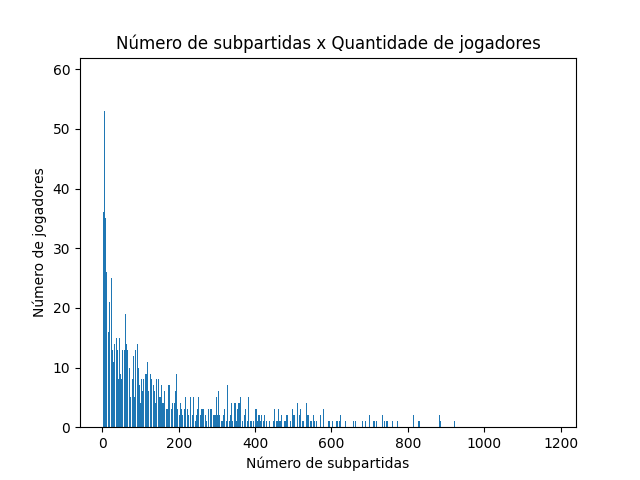
\includegraphics[scale = 0.8]{images/games_played_per_player.png}
    \caption{Número de jogadores conforme o número de subpartidas em que ele atuou.}
    \label{games_played}
\end{figure}

Para ilustrar a ideia da clusterização podemos ver a Figura \ref{games_played}, onde percebe-se que muitos atletas atuaram em poucas subpartidas. Nesse cenário, a função de log-verossimilhança permanece tendo a mesma forma que vimos previamente, a única alteração se dá na definição das forças de ataque e defesa de cada clube, as quais passam a se expressar como \ref{novos_lambdas}.
\begin{equation}
    \begin{split}
        \lambda_{m, a, g, k} & = \sum_{i} q_{i, m, g, k}\cdot p_{i, a}, \\
        \lambda_{v, a, g, k} & = \sum_{i} q_{i, v, g, k}\cdot p_{i, a}, \\
        \lambda_{m, d, g, k} & = \sum_{i} q_{i, m, g, k}\cdot p_{i, d} \text{ e} \\
        \lambda_{v, d, g, k} & = \sum_{i} q_{i, v, g, k}\cdot p_{i, d}.
    \end{split}
    \label{novos_lambdas}
\end{equation}

Essa clusterização, apesar de simples, reduz de modo considerável o número de parâmetros. Se utilizarmos como quantidade mínima 20 subpartidas, temos que o número de jogadores a serem utilizados para a modelagem é de 2547, contra os 3154 originais, o que corresponde a uma diminuição de aproximadamente 20\% no número de parâmetros a serem estimados. Nesse cenário, os jogadores com menos de 20 subpartidas são agrupados, sendo substituídos por 20 novos jogadores, cada um desses correspondendo ao conjunto de jogadores que jogou cada quantidade de subpartidas entre 1 e 20.

Outra agregação possível, agora em relação ao tempo de jogo, seria o agrupamento de jogadores com uma certa quantidade de minutos de jogo, a qual não será explorada no trabalho, mas que segue raciocínio análogo ao descrito acima.

Por fim, observe que se $q_{i, m, g, k}, q_{i, v, g, k} \in \{0, 1\}$ para todos os valores de $g$ e $k$ então estamos no caso anterior, onde a clusterização não foi aplicada, logo, essa é uma formulação mais geral que a inicial. Sendo assim, iremos utilizar esse modelo daqui em diante.

Apesar da clusterização juntar alguns atletas e diminuir o número de parâmetros a serem estimados, tal número permanece elevado. Nesse sentido, é interessante conhecer um pouco mais a função que desejamos otimizar. Para tanto, podemos calcular o gradiente da função, o qual pode auxiliar nos algoritmos de otimização. As derivadas parciais de $\mathcal{L}$ podem ser expressas por
\begin{equation*}
    \begin{split}
        \dfrac{\partial \mathcal{L}}{\partial p_{i, a}} & = \sum_{g}\sum_{k = 0}^{n_g} \left(-t_{g, k}\cdot \dfrac{q_{i, m, g, k}}{\lambda_{v, d, g, k}} + s_{m, g, k}\cdot \dfrac{q_{i, m, g, k}}{\lambda_{m, a, g, k}} -t_{g, k}\cdot \dfrac{q_{i, v, g, k}}{\lambda_{m, d, g, k}} + s_{v, g, k}\cdot \dfrac{q_{i, v, g, k}}{\lambda_{v, a, g, k}} \right) \text { e} \\
        \dfrac{\partial \mathcal{L}}{\partial p_{i, d}} & = \sum_{g}\sum_{k = 0}^{n_g} \left(t_{g, k}\cdot \dfrac{q_{i, v, g, k}\cdot \lambda_{m, a, g, k}}{\left(\lambda_{v, d, g, k}\right)^2} - s_{m, g, k}\cdot  \dfrac{q_{i, v, g, k}}{\lambda_{v, d, g, k}} + t_{g, k}\cdot \dfrac{q_{i, m, g, k}\cdot \lambda_{v, a, g, k}}{\left(\lambda_{m, d, g, k}\right)^2} - s_{v, g, k}\cdot \dfrac{q_{i, m, g, k}}{\lambda_{m, d, g, k}}\right),
    \end{split}
\end{equation*}

\noindent que, fatorando pela quantidade de aparições do jogador no intervalo de jogo, pode ser reescrito como em \ref{derivadas}.
\begin{equation}
    \begin{split}
        \dfrac{\partial \mathcal{L}}{\partial p_{i, a}} & = \sum_{g}\sum_{k = 0}^{n_g} \left(q_{i, m, g, k}\left(- \dfrac{t_{g, k}}{\lambda_{v, d, g, k}} + \dfrac{s_{m, g, k}}{\lambda_{m, a, g, k}}\right) + q_{i, v, g, k}\left(- \dfrac{t_{g, k}}{\lambda_{m, d, g, k}} + \dfrac{s_{v, g, k}}{\lambda_{v, a, g, k}}\right)\right) \text { e} \\
        \dfrac{\partial \mathcal{L}}{\partial p_{i, d}} & = \sum_{g}\sum_{k = 0}^{n_g} \left(q_{i, m, g, k}\left(\dfrac{t_{g, k}}{\lambda_{m, d, g, k}}\cdot \dfrac{\lambda_{v, a, g, k}}{\lambda_{m, d, g, k}} - \dfrac{s_{v, g, k}}{\lambda_{m, d, g, k}}\right) + q_{i, v, g, k}\left(\dfrac{t_{g, k}}{\lambda_{v, d, g, k}}\cdot \dfrac{\lambda_{m, a, g, k}}{\lambda_{v, d, g, k}} - \dfrac{s_{m, g, k}}{\lambda_{v, d, g, k}}\right)\right).
    \end{split}
    \label{derivadas}
\end{equation}

De onde podemos montar o vetor gradiente $\nabla \mathcal{L}$ como
\begin{equation*}
    \nabla_i \mathcal{L} = 
    \left\{
        \begin{array}{@{}l@{}}
            \dfrac{\partial \mathcal{L}}{\partial p_{i, a}}, \text{ se } i \leq n_p\\
            \dfrac{\partial \mathcal{L}}{\partial p_{i - n_p, d}}, \text{ c.c.}
        \end{array}
    \right.\,.
\end{equation*}

Além do gradiente, podemos buscar a hessiana de $\mathcal{L}$ e analisar a convexidade da função por meio da mesma, a qual é dada em \ref{derivadas_segunda}.
\begin{equation}
    \begin{split}
        \dfrac{\partial^2 \mathcal{L}}{\partial p_{i, a} \partial p_{j, a}} & = \sum_{g}\sum_{k = 0}^{n_g} \left(- q_{i, m, g, k}\cdot q_{j, m, g, k}\cdot \dfrac{s_{m, g, k}}{\lambda_{m, a, g, k}^2} - q_{i, v, g, k}\cdot q_{j, v, g, k}\cdot \dfrac{s_{v, g, k}}{\lambda_{v, a, g, k}^2}\right), \\
        \dfrac{\partial^2 \mathcal{L}}{\partial p_{i, d} \partial p_{j, a}} & = \sum_{g}\sum_{k = 0}^{n_g} \left(q_{i, m, g, k}\cdot q_{j, v, g, k}\cdot \dfrac{t_{g, k}}{\lambda_{m, d, g, k}^2} + q_{i, v, g, k}\cdot q_{j, m, g, k}\cdot \dfrac{t_{g, k}}{\lambda_{v, d, g, k}^2}\right), \\
        \dfrac{\partial^2 \mathcal{L}}{\partial p_{i, a} \partial p_{j, d}} & = \sum_{g}\sum_{k = 0}^{n_g} \left(q_{i, m, g, k}\cdot q_{j, v, g, k}\cdot \dfrac{t_{g, k}}{\lambda_{v, d, g, k}^2} + q_{i, v, g, k}\cdot q_{j, m, g, k}\cdot \dfrac{t_{g, k}}{\lambda_{m, d, g, k}^2}\right) \text { e} \\
        \dfrac{\partial^2 \mathcal{L}}{\partial p_{i, d} \partial p_{j, d}} & = \sum_{g}\sum_{k = 0}^{n_g} \left(q_{i, m, g, k}\cdot q_{j, m, g, k}\cdot \left(\dfrac{s_{v, g, k}}{\lambda_{m, d, g, k}^2} - \dfrac{2\cdot t_{g, k}\cdot \lambda_{v, a, g, k}}{\lambda_{m, d, g, k}^3}\right)\right) \\
        & ~~ + \sum_{g}\sum_{k = 0}^{n_g} \left(q_{i, v, g, k}\cdot q_{j, v, g, k}\cdot \left(\dfrac{s_{m, g, k}}{\lambda_{v, d, g, k}^2} - \dfrac{2\cdot t_{g, k}\cdot \lambda_{m, a, g, k}}{\lambda_{v, d, g, k}^3}\right)\right).
    \end{split}
    \label{derivadas_segunda}
\end{equation}

De modo análogo ao gradiente, podemos definir a matriz hessiana $\nabla^2 \mathcal{L}$ de forma matricial por meio das expressões de \ref{derivadas_segunda}.
\begin{equation*}
    \nabla_{i, j}^2 \mathcal{L} = 
    \left\{
        \begin{array}{@{}l@{}}
            \dfrac{\partial^2 \mathcal{L}}{\partial p_{i, a} \partial p_{j, a}}, \text{ se } i \leq n_p \text{ e } j \leq n_p \\
            \dfrac{\partial^2 \mathcal{L}}{\partial p_{i, a} \partial p_{j - n_p, d}}, \text{ se } i \leq n_p \text{ e } j > n_p \\
            \dfrac{\partial^2 \mathcal{L}}{\partial p_{i - n_p, d} \partial p_{j, a}}, \text{ se } i > \text{ e } j \leq n_p \\
            \dfrac{\partial^2 \mathcal{L}}{\partial p_{i - n_p, d} \partial p_{j - n_p, d}}, \text{ se } i > \text{ e } j > n_p
        \end{array}
    \right.\,.
\end{equation*}

Por fim, para verificar a convexidade de $\mathcal{L}$ devemos ter que $\nabla^2 \mathcal{L}$ deve ser semi-definida positiva. Mas isso não é verdadeiro, visto que tomando qualquer vetor canônico $e_l$, temos que $e_l^\top\cdot \nabla^2 \mathcal{L}\cdot e_l = \nabla_{l, l}^2 \mathcal{L}$. Agora, escolhendo $l \leq n_p$, temos que
\begin{equation*}
    \begin{split}
        \nabla_{l, l}^2 \mathcal{L} & = \sum_{g}\sum_{k = 0}^{n_g} \left(- q_{l, m, g, k}^2\cdot \dfrac{s_{m, g, k}}{\lambda_{m, a, g, k}^2} - q_{l, v, g, k}^2\cdot \dfrac{s_{v, g, k}}{\lambda_{v, a, g, k}^2}\right) \\
        & = - \sum_{g}\sum_{k = 0}^{n_g} \left(q_{l, m, g, k}^2\cdot \dfrac{s_{m, g, k}}{\lambda_{m, a, g, k}^2} + q_{l, v, g, k}^2\cdot \dfrac{s_{v, g, k}}{\lambda_{v, a, g, k}^2}\right),
    \end{split}
\end{equation*}

\noindent é um número negativo ou nulo, visto que os termos quadráticos são não negativos e os valores de $s_{m, g, k}$ e $s_{v, g, k}$ são correspondentes ao placar do jogo, logo também são não negativos.

Dessa forma, se escolhermos $l$ de modo que esse vetor corresponda a direção de um jogador que entrou em campo em, pelo menos, uma subpartida que não terminou zero a zero temos que $e_l^\top\cdot \nabla^2 \mathcal{L}\cdot e_l < 0$, o que mostra que $\nabla^2 \mathcal{L}$ não é semi-definida positiva e, consequentemente, que $\mathcal{L}$ não é convexa.

Apesar da não convexidade de $\mathcal{L}$, foi elaborado um código em Python que, por meio da biblioteca \path{scipy}, busca os parâmetros que otimizam a função de verossimilhança. Foram testados diversos algoritmos para otimização, com e sem a utilização do gradiente e da hessiana, além de se valer da clusterização, onde os jogadores com até 20 subpartidas foram agrupados. Entretanto, em virtude da não convexidade e do espaço de parâmetros, que ainda possui uma dimensão alta, a otimização ainda se mostrou complexa. Diante do exposto, optou-se por deixar a abordagem frequentista de lado e se voltar a abordagem bayesiana.

\section{Abordagem Bayesiana}

Alternativamente a abordagem frequentista, apresentada na seção anterior, podemos modelar o futebol através do paradigma bayesiano. Nessa abordagem cada jogador continua sendo definido por um conjunto de parâmetros, porém tais parâmetros não são mais valores reais fixos, mas sim variáveis aleatórias. Com isso em mente, o objetivo passa, da estimação dos parâmetros de cada jogador, para a estimação da distribuição de probabilidade de cada uma dessas variáveis que representam os jogadores. Para tanto, necessitamos de um modelo e também de uma hipótese, à priori, de como os parâmetros das distribuições que modelam as observações se comportam.

Seguindo essa linha de pensamento, podemos, primeiramente, definir um modelo.

\subsection{ADM - Attack and Defense Model}
\label{ADM_text}

Para a modelagem inicial dessa abordagem, iremos nos valer do modelo de Poisson descrito na seção anterior, isso é, onde os gols em uma subpartida são expressos pelas equações em \ref{ADM_model}. Já os valores de $\lambda_{m,a,g,k}$, $\lambda_{v,a,g,k}$, $\lambda_{m,d,g,k}$ e $\lambda_{v,d,g,k}$, os quais, na abordagem frequentista, foram tomados como em \ref{novos_lambdas} (uma generalização de \ref{lambdas}), são definidos de modo análogo, bastando definir se a clusterização, explicada e utilizada na seção anterior, será ou não aplicada a este modelo. Para essa modelagem, a mesma não foi utilizada, de modo que definimos tais valores conforme as Equações em \ref{lambdas}. Novamente, devemos lembrar que não faz sentido termos valores negativos para as proficiências dos jogadores, pois isso implicaria numa piora do desempenho do time com tal jogador em campo em relação a quando o time joga com um jogador a menos.

Com o modelo definido, passamos a elicitação da nossa hipótese à priori. Aqui, como cada jogador é dado por uma distribuição, é inviável definir, manualmente, priori por priori. Algumas possibilidades são plausíveis para elicitação das mesmas, como a utilização do valor de mercado dos jogadores ou do clube em que os mesmos atuam como forma de balancear os jogadores inicialmente.

Tais ideias partem das premissas de que, no caso da primeira, jogadores mais caros são, em geral, melhores. Para a segunda ideia, adicionamos a premissa de que os jogadores de um mesmo clube tendem a ter desempenhos similares. Assim, juntando com a premissa utilizada na primeira ideia, teríamos que a qualidade técnica de todos os jogadores de um time deve ser similar, logo, o valor de mercado do clube poderia ser a base da priori para todos os jogadores. Naturalmente, há exceções. Jogadores que jogam em mercados com menor visibilidade tendem a ter preços menores, uma vez que são pouco observados.

Essas prioris são razoáveis (os valores de mercado são sempre positivos) e podem ser utilizadas com facilidade por meio de dados do Transfermarkt \cite{transfermarkt}. Entretanto, para o escopo desse trabalho, foi utilizada a mesma priori para todos os jogadores, de modo que, apesar da falta de informação inicial, facilitará na implementação do modelo. Nesse sentido, a priori utilizada foi uma distribuição semi-normal, isso é, a distribuição de $Y = |X|$, sendo $X\sim N(0, 1)$. Ou, por simplicidade de implementação, uma normal padrão truncada em zero.

Essa priori, além de poder ter a interpretabilidade de que os atletas possuem um nível de habilidade dado por uma normal, poderia facilitar algumas contas ao realizar os cálculos de modo analítico. Sabendo que a verossimilhança do modelo proposto é dada por uma Poisson, ter uma priori Gamma para o parâmetro da Poisson pode nos dar, diretamente, a posteriori. Como a priori dada é semi-normal, o parâmetro da Poisson tomada como verossimilhança será uma variável aleatória Chi-quadrado, a qual é um caso especial da Gamma, pois se dá pela razão de somas de variáveis semi-normais. Dessa forma, os cálculos analíticos podem ser simplificados.

Entretanto, dado o número elevado de jogos e jogadores a serem modelados, optou-se pelo uso do algoritmo HMC por meio do Stan \cite{stan}, de modo a obter as amostras das distribuições à posteriori dos parâmetros de interesse ao invés de calculá-los analiticamente. Com o modelo e a priori definida partiu-se para a implementação do modelo, o qual está disponível no Apêndice \ref{stan_model_1}.

Como entrada, o modelo recebe informações sobre o número de subpartidas que estão sendo modeladas, bem como o número de jogadores e o vetor de tempo de cada uma das subpartidas. Além disso, temos o número de jogadores por clube em cada uma das subpartidas, apenas para possibilitar a criação dos \textit{arrays} para cada um dos clubes. Por fim, os últimos três dados de entrada são referentes aos dados observados de fato, isso é, os placares de cada uma das subpartidas e cada uma das escalações (mandante e visitante), também para cada uma das subpartidas.

A definição dos parâmetros e do modelo leva em consideração o que desejamos amostrar. Como queremos amostrar as distribuições de $p_{i, a}$ e de $p_{i,d}$ para todos os possíveis jogadores $i$, os parâmetros do modelo se referem justamente a isso, onde cada um dos vetores corresponde a uma dessas forças. Como comentado previamente, tais parâmetros tem suporte nos reais positivos, o que também já foi restrito na definição dos parâmetros.

Por fim, o modelo deve receber uma priori para cada um dos parâmetros, a qual, como discutido anteriormente, é dada por uma semi-normal. Uma vez que os parâmetros já estão restritos a $\mathds{R}_+$, podemos considerar que a priori é dada por uma normal padrão. Além da priori, o modelo deve possuir uma função de verossimilhança para que o mesmo possa realizar o cálculo da distribuição, a qual é dada conforme o modelo em \ref{ADM_model}.

\subsection{HAM - Home Away Model}

Agora, com um primeiro modelo definido, podemos voltar a Figura \ref{goals_graph}, onde temos os histogramas de gols de cada partida, discriminados pelo mando de campo. Apesar do teste de hipóteses realizado, cujos resultados foram apresentados na Tabela \ref{hyp_test}, falhar em rejeitar a hipótese de que o número de gols em uma partida de futebol é dada por uma distribuição de Poisson, não temos a informação acerca do número de gols do mandante e do visitante serem dados pela mesma distribuição. Podemos ver que a mesma figura nos mostra que as médias dos gols é diferente em relação ao mando. Dessa forma, podemos questionar se há diferença entre a distribuição de gols do mandante para o visitante, isso é, o mandante possui alguma vantagem ou desvantagem em relação ao visitante? Essa pergunta é equivalente a nos perguntarmos acerca da igualdade entre as médias das distribuições que estamos modelando.

A resposta para essa pergunta é incerta, mas podemos levantar a hipótese de que duas as médias são iguais, ou seja, nenhum dos times possui vantagem. Nesse cenário, teríamos $s_{m, g, k}, s_{v, g, k} \sim \operatorname{Poisson}(\lambda)$, para algum $\lambda$. Para testar essa hipótese, podemos realizar um teste t de Student para média de duas amostras, já implementado na biblioteca \path{scipy}, a qual retorna a estatística de teste e o p-valor do teste. Para esse teste utilizaremos $\alpha = 0.01$, logo, se o p-valor retornado pela função ao receber as duas séries de gols for menor que $\alpha$, rejeitamos a hipótese nula, o que pode ser interpretado como uma evidência de que, ao menos minimamente, os times são influenciados pelo mando de campo.

Realizando o teste encontramos um p-valor de, aproximadamente, $9.852\cdot 10^{-51}$, o que nos faz rejeitar a hipótese de que as duas distribuições possuem médias iguais. Uma vez que tal hipótese foi rejeitada, podemos pensar em realizar algumas pequenas alterações no modelo de modo que possamos diferenciar o fator mando de campo. Duas modelagens surgem naturalmente, uma em que cada jogador possui um rendimento diferente conforme o mando de campo, isso é, o jogador $i$ tem rendimento $X$ jogando em casa e $Y$ jogando fora, ou onde cada clube possui um fator mando de campo, como se sua torcida fosse o décimo segundo jogador. Tais modelos podem ser definidos, matematicamente, por meio de pequenas alterações no modelo dado em \ref{ADM_model}.

\subsubsection{HAM1}
\label{HAM1_text}

Partindo para a modelagem dos jogadores junto ao mando de campo podemos considerar, primeiramente, o modelo em que os jogadores possuem rendimentos distintos conforme o local da partida (se o jogo é em casa ou fora). Nesse sentido, o modelo proposto previamente pode servir como modelo base e, por meio de pequenas alterações, podemos chegar ao modelo desejado.

Como a diferença entre tais modelos se dá pelo rendimento dos atletas conforme o mando de campo, a mudança natural é na inclusão de um novo conjunto de parâmetros para os jogadores, onde discrimina-se o mando. Dessa forma, os parâmetros $p_{i, a}$ e $p_{i, d}$ dão lugar aos parâmetros $p_{{i, a}_m}$, $p_{{i, d}_m}$, $p_{{i, a}_v}$ e $p_{{i, d}_v}$, os quais possuem a mesma interpretação dos parâmetros originais, mas incorporando a discriminação do mando. Com a alteração dos parâmetros dos jogadores, é natural que as forças dos clubes também se alterassem, de modo que, para esse modelo, os parâmetros dos clubes passam a ser expressos pelo conjunto de Equações \ref{lambdas_HAM1}.
\begin{equation}
    \begin{split}
        \lambda'_{m, a, g, k} & = \sum_{i \in \mathcal{C}_{m, g, k}} p_{{i, a}_m}, \\
        \lambda'_{v, a, g, k} & = \sum_{i \in \mathcal{C}_{v, g, k}} p_{{i, a}_v}, \\
        \lambda'_{m, d, g, k} & = \sum_{i \in \mathcal{C}_{m, g, k}} p_{{i, d}_m} \text{ e} \\
        \lambda'_{v, d, g, k} & = \sum_{i \in \mathcal{C}_{v, g, k}} p_{{i, d}_v},
    \end{split}
    \label{lambdas_HAM1}
\end{equation}

Finalmente, o modelo final possui a mesma forma do modelo anterior, sendo dado por \ref{HAM1_model}.
\begin{equation}
    \begin{split}
    s_{m, g, k} & \sim \operatorname{Poisson}\left(\dfrac{\lambda'_{m,a,g,k}}{\lambda'_{v,d,g,k}} \cdot t_{g,k}\right) \\
    s_{v, g, k} & \sim \operatorname{Poisson}\left(\dfrac{\lambda'_{v,a,g,k}}{\lambda'_{m,d,g,k}} \cdot t_{g,k}\right),
    \end{split}
    \label{HAM1_model}
\end{equation}

Novamente, utilizando uma priori semi-normal para os parâmetros dos jogadores, podemos elaborar o código Stan para tal modelo. O código, assim como no modelo anterior, está disponível no Apêndice \ref{stan_model_2}. Como o modelo propriamente dito, a implementação também é bem similar a anterior, havendo apenas a alteração dos parâmetros e, consequentemente, da média da Poisson.

\subsubsection{HAM2}
\label{HAM2_text}

Por fim, além de modelar a diferença que o mando de campo gera por meio dos jogadores, pode-se realizar tal  modelagem de modo que essa diferença seja explicada por meio do clube mandante. Nesse caso, cada clube possui um parâmetro que diferencia sua atuação em casa para a atuação fora de casa, servindo, literalmente, como um décimo segundo jogador. Desse modo, o mando de campo terá influência para melhorar tanto o ataque quanto a defesa do clube mandante. Matematicamente, podemos traduzir essa ideia por meio do modelo em \ref{HAM2_model}.
\begin{equation}
    \begin{split}
    s_{m, g, k} & \sim \operatorname{Poisson}\left(\left(\dfrac{\lambda_{m,a,g,k} + \kappa_{m,a,g,k}}{\lambda_{v,d,g,k}}\right) \cdot t_{g,k}\right) \\
    s_{v, g, k} & \sim \operatorname{Poisson}\left(\left(\dfrac{\lambda_{v,a,g,k}}{\lambda_{m,d,g,k} + \kappa_{m,d,g,k}}\right) \cdot t_{g,k}\right).
    \end{split}
    \label{HAM2_model}
\end{equation}

Os valores de $\lambda_{m,a,g,k}$, $\lambda_{v,a,g,k}$, $\lambda_{m,d,g,k}$ e $\lambda_{v,d,g,k}$ foram tomados como em \ref{novos_lambdas}, enquanto $\kappa_{m,a,g,k}$ e $\kappa_{m,d,g,k}$ são novos parâmetros, também com suporte em $\mathds{R}_+$.

Por meio do Modelo \ref{HAM2_model}, podemos ver que o mando de campo se encaixa exatamente como mais um jogador para o clube mandante, o que nos permite ver com maior clareza a possibilidade que esse fator tem de neutralizar a equipe adversária. Entretanto, também por meio dessas equações, pode-se ver que a efetividade do mando de campo também depende do adversário, isso é, o mando de campo por si só não garante que o clube mandante irá ter um determinado resultado.

Novamente, tal modelo foi implementado no Stan tendo como base o código inicial, do modelo ADM. O código final para esse modelo pode ser visto no Apêndice \ref{stan_model_3}.

Para tal modelo, além dos dados que o modelo ADM utiliza, necessitamos inserir o número de clubes que estão sendo modelados e um \textit{array} mapeando o clube mandante de cada uma das partidas. As demais alterações no código são referentes aos parâmetros que serão estimados, os quais foram incluídos no modelo. Mais uma vez, atribuiu-se uma priori de distribuição semi-normal aos mesmos. Por fim, foram realizadas alterações na média da Poisson para que a mesma correspondesse ao modelo desejado.

Por fim, vale lembrar que tais modelos sofrem com um problema de identificabilidade, ou seja, assim como visto na Seção \ref{abordagem_frequentista}, multiplicar ou dividir todos os parâmetros não irá alterar os modelos.

\subsection{Rodando os modelos}

Após definir os modelos podemos realizar a execução dos mesmos, obtendo amostras das distribuições a posteriori dos parâmetros dos jogadores. Devemos lembrar que o número de jogadores modelados, bem como o de subpartidas, é muito grande, logo tais execuções são custosas. Além disso, por se tratar de algoritmos que usam cadeias de Markov, as paralelizações possíveis são na execução simultânea de diferentes cadeias para cada um dos modelos, entretanto isso também detém um custo computacional. Nesse sentido, com o intuito de otimizar a execução, driblando o custo computacional, utilizou-se, assim como no processo de raspagem, o GitHub Actions para executar o modelo.

\subsubsection{Resultados}

Tendo rodado os modelos, podemos partir para a análise dos resultados. Os principais resultados serão acerca dos melhores jogadores de modo geral. Para tanto, podemos ranquear os jogadores por meio do produto de suas proficiências, assim, quanto maior o produto, melhor sua posição no ranking. Essa métrica, derivada da média geométrica, auxilia a traduzir o impacto de cada jogador em uma subpartida. Tal impacto pode ser visto por meio da média da distribuição de gols. Para o número de gols do seu clube atacante, a variação da proficiência de ataque de um jogador, aumentando sua proficiência, influencia positivamente a média, fazendo com que a mesma aumente. Por outro lado, em relação ao número de gols do adversário, o aumento da proficiência de defesa de um jogador faz com que a média de gols do seu adversário diminua, uma vez que esse parâmetro aparece no denominador.

Para elaboração desse ranking, a proficiência de ataque e de defesa utilizada será a proficiência média da distribuição amostrada para cada jogador. Em relação ao modelo HAM2, o qual possui duas forças de ataque e duas de defesa para cada jogador, as proficiências utilizadas se dão pela média de todas as proficiências de ataque e pela média de todas as proficiências de defesa.

Os melhores jogadores do período de 2018 a 2022, segundo essa métrica, podem ser vistos na Tabela \ref{ranking}.
\begin{table}[H]
    \centering
    \begin{tabular}{c|rrr}
        \hline
        Pos. & ADM               & HAM1               & HAM2              \\ \hline
        1    & Sávio (VIL/GO)    & Gustavo (OES/SP)   & Vitinho (GUA/SP)  \\
        2    & Bruno (NOV/SP)    & Tiago C. (BOT/SP)  & Maicon (BRA/RS)   \\
        3    & Vitinho (GUA/SP)  & Marlon (OES/SP)    & Bruno (NOV/SP)    \\
        4    & Henrique (CSA/AL) & Werik (RBB/SP)     & Rincon (CUI/MT)   \\
        5    & Maicon (BRA/RS)   & Caue (JUV/RS)      & Sávio (VIL/GO)    \\
        6    & Leandro (OPE/PR)  & Landazuri (FOR/CE) & Leandro (OPE/PR)  \\
        7    & Fernando (LON/PR) & Leo Bahia (BRA/RS) & Fernando (LON/PR) \\
        8    & Lessa (BOT/RJ)    & Leonardo (INT/RS)  & Sávio (CAM/MG)    \\
        9    & Sávio (CAM/MG)    & Bruno (GUA/SP)     & Lessa (BOT/RJ)    \\
        10   & Darli (CRB/AL)    & Vladimir (AVA/SC)  & Darli (CRB/AL)    \\ \hline
    \end{tabular}
    \caption{Ranking: Melhores jogadores segundo cada modelo.}
    \label{ranking}
\end{table}

Note que os rankings dos modelos ADM e HAM2 são bem parecidos, com apenas um jogador diferente, exceto pela ordem. Isso é razoável, uma vez que os modelos são similares, se alterando apenas por meio do fator mando de campo, o qual, no modelo HAM2, atua como um jogador a mais. Além disso, muitos desses jogadores atuam em clubes de menor expressão, como Sávio, no Vila Nova, e Vitinho, no Guarani, onde possivelmente também devem ter atuado pouco. Uma forma de lidar com esse problema é filtrar os jogadores, de modo que só entrem para o ranking os atletas que participaram de, ao menos, 100 subpartidas. Nesse sentido, podemos elaborar o ranking visto na Tabela \ref{ranking2}.
\begin{table}[H]
    \centering
    \begin{tabular}{c|rrr}
        \hline
        Pos. & ADM                  & HAM1                & HAM2                 \\ \hline
        1    & Wellington (ATL/GO)  & Juninho (AME/MG)    & Wellington (ATL/GO)  \\
        2    & Ricardo (CRB/AL)     & Sornoza (COR/SP)    & Giuliano (COR/SP)    \\
        3    & Wellington (AME/MG)  & Jarro (BRA/RS)      & Ricardo (CRB/AL)     \\
        4    & Giuliano (COR/SP)    & Léo Artur (SAM/MA)  & Daniel (BOT/RJ)      \\
        5    & Igor Carius (CUI/MT) & Ramon (ATL/GO)      & Wellington (AME/MG)  \\
        6    & Daniel (BOT/RJ)      & Rayan (CRI/SC)      & Igor Carius (CUI/MT) \\
        7    & Sornoza (COR/SP)     & Matheus (CEA/CE)    & Sornoza (COR/SP)     \\
        8    & Mansur (SAO/SP)      & Roni (COR/SP)       & Mansur (SAO/SP)      \\
        9    & Leo (CHA/SC)         & Wellington (AME/MG) & Augusto (LON/PR)     \\
        10   & Tadeu (GOI/GO)       & Tadeu (GOI/GO)      & Leo (CHA/SC)         \\ \hline
    \end{tabular}
    \caption{Ranking: Melhores jogadores, com pelo menos 100 subpartidas disputadas, segundo cada modelo.}
    \label{ranking2}
\end{table}

Podemos ver que, novamente, os rankings do ADM e do HAM2 são bem similares. Além disso, já aparecem mais jogadores conhecidos. Dois jogadores que chamam atenção nesse ranking são o Wellington, do América Mineiro, e Sornoza, ex-jogador do Corinthians, os quais aparecem no ranking de todos os modelos. Dado isso, podemos ver como sua distribuição se comporta, iteração a iteração da Cadeia de Markov, conforme Figuras \ref{plots1} e \ref{plots2}.
\begin{figure}[H]
    \subfloat[AMD - Wellington.]{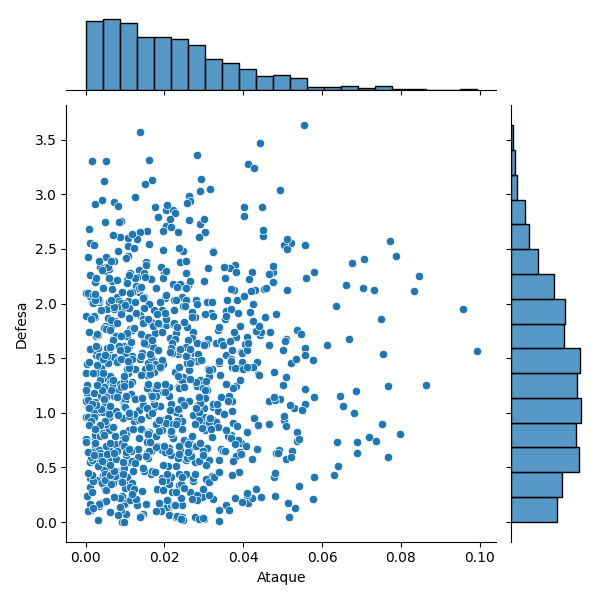
\includegraphics[width = 3in]{images/players/ADM_152788.png}} 
    \subfloat[AMD - Sornoza.]{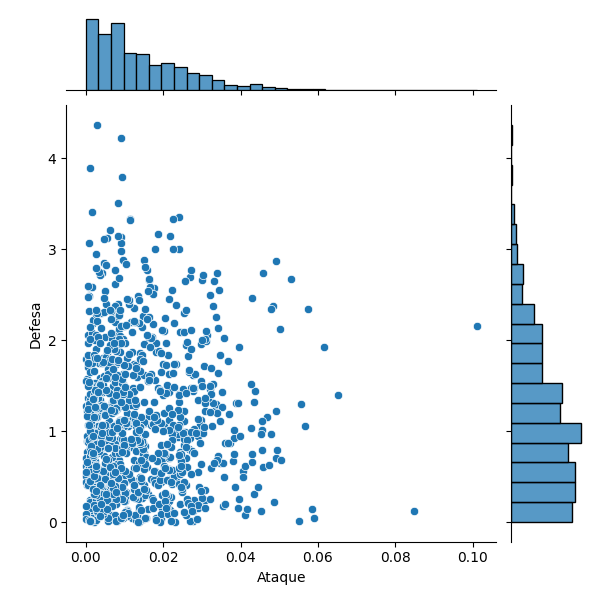
\includegraphics[width = 3in]{images/players/ADM_565315.png}}
    \caption{Distribuições ADM - Wellington e Sornoza.}
    \label{plots1}
\end{figure}

\begin{figure}
    \subfloat[HAM1 - Wellington.]{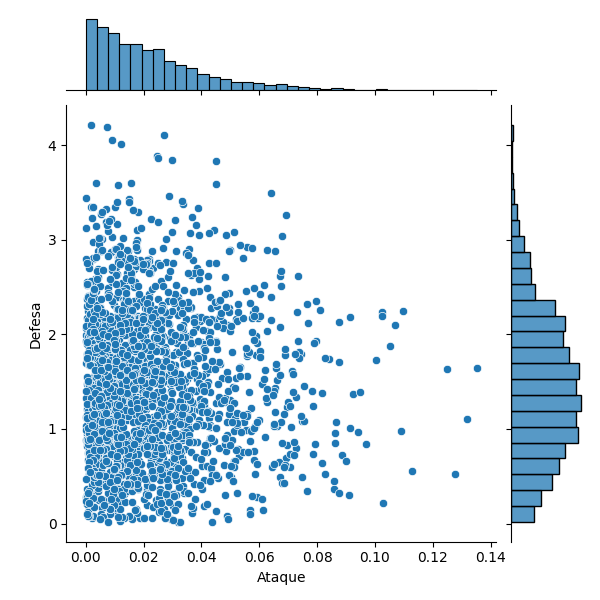
\includegraphics[width = 3in]{images/players/HAM1_152788.png}}
    \subfloat[HAM1 - Sornoza.]{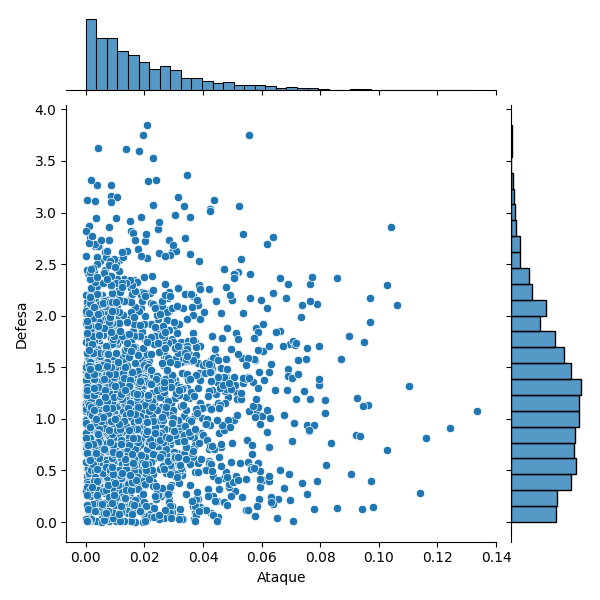
\includegraphics[width = 3in]{images/players/HAM1_565315.png}}\\
    \subfloat[HAM2 - Wellington.]{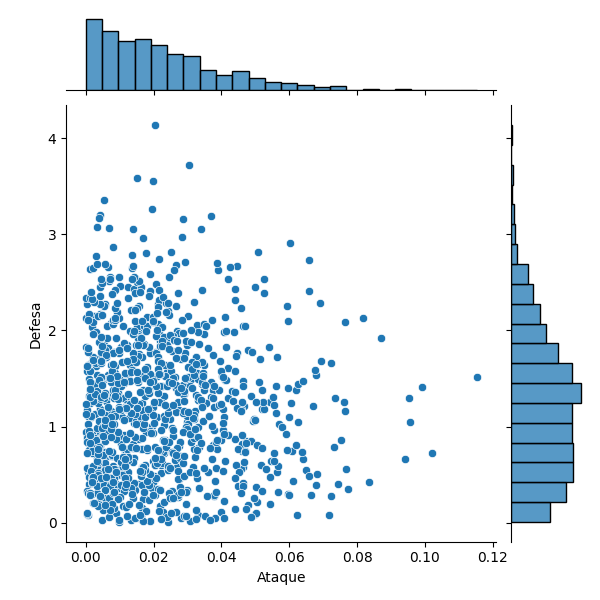
\includegraphics[width = 3in]{images/players/HAM2_152788.png}}
    \subfloat[HAM2 - Sornoza.]{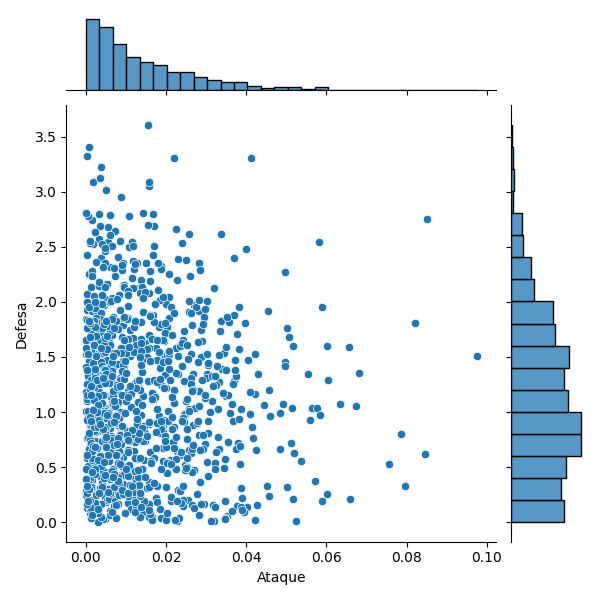
\includegraphics[width = 3in]{images/players/HAM2_565315.png}} 
    \caption{Distribuições HAM - Wellington e Sornoza.}
    \label{plots2}
\end{figure}

Pode-se ver que as distribuições são similares. Além disso, os parâmetros defensivos possuem valores muito mais elevados que os parâmetros ofensivos, o que já era esperado. Visto que, em todos os modelos, a média da distribuição de Poisson é dada pelo produto entre a razão entre as forças das equipes e o tempo de jogo, podemos interpretar tal razão como a média de gols em um minuto. Como o número de gols esperados em um minuto dentro de um jogo de futebol é muito baixo, faz sentido que os parâmetros defensivos sejam maiores que os ofensivos.

Outra análise interessante é a de comparar qual jogador é melhor. Nesse sentido pode-se comparar, por exemplo, dois atacantes da dupla Fla-Flu: Pedro e Germán Cano. Como ambos são jogadores referência no ataque, atuando como centroavante, seus parâmetros de defesa podem ser desconsiderados para a avaliação, uma vez que a ideia é ver quem contribui mais para fazer gols. Dessa forma, podemos ilustrar, graficamente, a distribuição dos parâmetros ofensivos de cada um dos dois atletas. Novamente, devemos lembrar do problema de identificabilidade do modelo, logo podemos fazer uma padronização em tais parâmetros, de modo que a média do parâmetro ofensivo do atacante tricolor seja fixada em 1 com o intuito de melhorar a escala para a visualização. No caso do HAM1, a normalização se dá, apenas, na proficiência de ataque em casa.
\begin{figure}[H]
    \subfloat[AMD.]{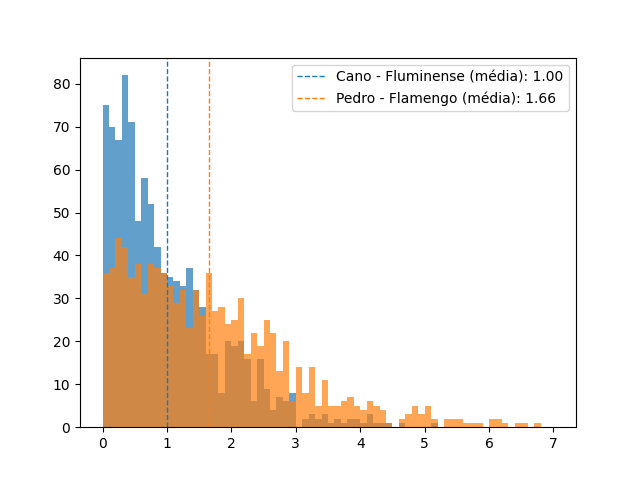
\includegraphics[width = 3.1in]{images/strikers_18B_ADM_atk.png}} 
    \subfloat[HAM2.]{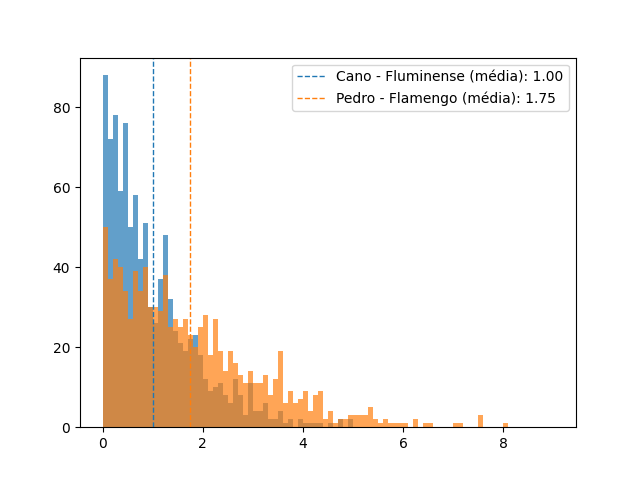
\includegraphics[width = 3.1in]{images/strikers_18B_HAM2_atk.png}}\\
    \subfloat[HAM1 - casa.]{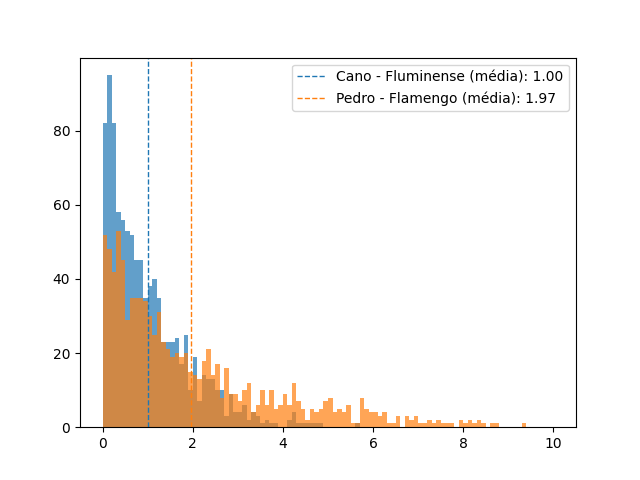
\includegraphics[width = 3.1in]{images/strikers_18B_HAM1_atk_home.png}}
    \subfloat[HAM1 - fora.]{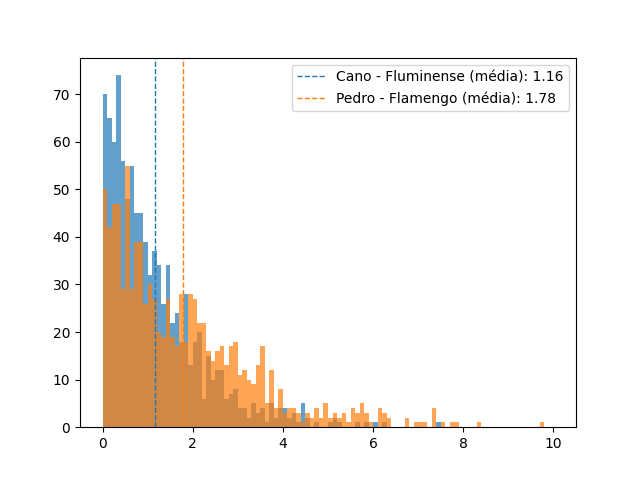
\includegraphics[width = 3.1in]{images/strikers_18B_HAM1_atk_away.png}}
    \caption{Distribuições ofensivas: Germán Cano e Pedro no período de 2018 a 2022.}
    \label{plots3}
\end{figure}

Conforme Figura \ref{plots3}, pode-se ver que, segundo o HAM1, jogando em casa Pedro é, em média, quase duas vezes mais eficiente que Germán Cano. Por outro lado, quando estão fora de seus domínios, Germán Cano é um pouco mais efetivo, enquanto Pedro diminui seu rendimento, o que faz a diferença entre eles diminuir um pouco, mas ainda com vantagem considerável para o atacante flamenguista. Em relação aos outros dois modelos, Pedro também se mostra mais efetivo, com margens, em relação a média, similares.

Por fim, além do ranking de jogadores, o HAM2 nos possibilita ranquear os clubes. Tal ranking pode ser elaborado de modo análogo ao dos jogadores, por meio da comparação dos produtos entre a média da distribuição ofensiva e defensiva que, no caso dos clubes, podem ser interpretados como o quanto a torcida (ou algum outro fator) influencia apoiando o clube, tanto no setor ofensivo quanto no defensivo. Dessa forma, considerando o período de 2018 a 2022, os clubes com o maior impacto podem ser encontrados na Tabela \ref{rankig_clubs}.
\begin{table}[H]
    \centering
    \begin{tabular}{r|c}
        \hline
        Pos. & Clube \\ \hline
           1 &            Joinville / SC \\
           2 &                Icasa / CE \\
           3 &           Mogi Mirim / SP \\
           4 &            Vila Nova / GO \\
           5 & Athletico Paranaense / PR \\
           6 &                 Avaí / SC \\
           7 &                  ABC / RN \\
           8 &                  CRB / AL \\
           9 &          São Caetano / SP \\
          10 &             Paysandu / PA \\ \hline
    \end{tabular}
    \caption{Ranking dos clube com maior influência do mando de campo.}
    \label{rankig_clubs}
\end{table}

Como pode-se ver, alguns clubes de menor expressão, predominantemente clubes que jogaram a série B nesse período, tomam conta das primeiras posições do ranking. Tal posicionamento faz sentido, uma vez que, muitas vezes, clubes da série B possuem um orçamento menor, além de maiores problemas logísticos o que pode acarretar na piora do seu desempenho nas partidas que joga como visitante. Consequentemente, o desempenho como mandante do seu adversário tende a melhorar, fato que reflete no parâmetro $\kappa$ desses clubes.

Um clube que vai à contramão da ideia apresentada no parágrafo anterior é o Athletico Paranaense, que figura na quinta posição. Novamente, sua posição tem uma explicação plausível: o Athletico, até 2020, era o único clube que utilizava a grama sintética. Logo, jogar na Arena da Baixada era, muitas vezes um desafio um pouco maior para os adversários, acostumados com o gramado natural. De modo análogo, o Athletico enfrentava um desafio um pouco fora do habitual ao jogar fora de casa, o que pode explicar sua aparição nesse ranking.